\documentclass[12pt]{article} % Default font size is 12pt, it can be changed here

\usepackage[margin=1in]{geometry} % Required to change the page size to A4
\geometry{a4paper} % Set the page size to be A4 as opposed to the default US Letter

\usepackage{abstract, adjustbox, amsmath, amssymb, array, indentfirst, fancyhdr, float, listings, longtable, multicol, multirow, natbib, parskip, setspace, tabu, tabularx, tikz, titlesec, verbatim, xcolor}
\usepackage{eso-pic, atbegshi, pdflscape, dcolumn}
\usepackage{ifthen, calc}
\usepackage{wrapfig, lipsum}
\usepackage{booktabs, tabularx, rotating}
\usepackage{listings}
\usepackage{indentfirst}
\usepackage{pdfpages}
\usepackage{graphicx}
\usepackage[format=plain,up,textfont=normal,up,justification=centering,singlelinecheck=false]{caption}   
\usepackage[bottom, hang, flushmargin]{footmisc}
\setlength{\headheight}{22pt}
\lstset{basicstyle=\ttfamily, columns=flexible, breaklines=true}
\PassOptionsToPackage{hyphens}{url}
\usepackage[colorlinks=false, hidelinks]{hyperref}
\onehalfspacing

\begin{document}
	
\setlength{\parindent}{0.5cm}
\parskip=0pt
\setcitestyle{aysep={}}

%----------------------------------------------------------------------------------------
%	TITLE PAGE
%----------------------------------------------------------------------------------------

\begin{titlepage}

\newcommand{\HRule}{\rule{\linewidth}{0.5mm}} % Defines a new command for the horizontal lines, change thickness here

\centering

\textsc{\LARGE University of Maryland}\\[1.5cm] % Name of your university/college
\textsc{\Large College of Behavioral and Social Sciences}\\[0.5cm] % Major heading such as course name
\textsc{\large Department of Government and Politics}\\[0.5cm] % Minor heading such as course title

\HRule \\[1.5cm]
{ \huge \bfseries Super Clumsy Title}\\[1cm] % Title of your document
\HRule \\[1.5cm]

\begin{minipage}{0.4\textwidth}
\begin{flushleft} \large
\emph{Author:}\\
Leo H. M. \textsc{Bauer} % Your name
\end{flushleft}
\end{minipage}
~
\begin{minipage}{0.4\textwidth}
\begin{flushright} \large
\emph{Supervisor:} \\
Prof. John \textsc{Smith} % Supervisor's Name
\end{flushright}
\end{minipage}\\[4cm]

{\large \today}\\[3cm] % Date, change the \today to a set date if you want to be precise

%\includegraphics{Logo}\\[1cm] % Include a department/university logo - this will require the graphicx package

\vfill % Fill the rest of the page with whitespace

\end{titlepage}

%----------------------------------------------------------------------------------------
%	TABLE OF CONTENTS
%----------------------------------------------------------------------------------------

\tableofcontents % Include a table of contents

\pagebreak

\listoftables

\listoffigures

\newpage % Begins the essay on a new page instead of on the same page as the table of contents 

\section{Introduction}

\noindent Anecdotes like this one illustrate how states are born in the world of nation-states as we know it since the Westphalian peace of 1648. 

\subsection{The Puzzle}

But although this episode in American history nears its 250th anniversary, the behavior of actors aspiring to become states has not much changed since then. 

\subsubsection{Research Question}

Purely $\rightarrow$ rationalist and structuralist explanations are still prevalent, but conflict scholars now increasingly argue that there is a link between compliance with international norms of statehood and the behavior of certain non-state actors: Just like Franklin on behalf of the Second Continental Congress, rebel groups that wish to secede from an existing nation-state to determine their own destiny mimic states' behavior in the international system and towards the domestic population in order to garner recognition and material support. 

\paragraph{Overview}

Moreover, the study of rebel behavior has become more relevant since the end of the cold war, replacing great power competition as one of the main fields of research in security and conflict studies. 

\subparagraph{Small Overview} 

This development has also been furthered by more precise data to study civil wars at both the dyadic and individual level. 

\pagebreak

Moreover, the study of rebel behavior has become more relevant since the end of the cold war, replacing great power competition as one of the main fields of research in security and conflict studies. \\ \

In this article, I thus pose the question of whether the behavioral phenomenon of secessionism in civil war can be extended to rebels' treatment of civilians in civil war. \bigskip 

Specifically, I argue that secessionist rebels are responsible for fewer civilian deaths than nonsecessionist rebels in civil war. \medskip 

Furthermore, I hypothesize that this effect remains stable or increases when these groups control territory. \smallskip 

To test these hypotheses, I use data from Stewart and the Uppsala Conflict Data Program (UCDP). \\ \

\textbf{The statistical results support my first hypothesis: Secessionist rebels are responsible for significantly fewer civilian fatalities than nonsecessionist rebels.} \\ \
	
\textit{However, I could not find statistically significant support for my second hypothesis.} \\ \

The variable {\footnotesize{CIVILIAN DEATHS}} is taken from the UCDP and has a negative binominal distribution. \\ \

\begin{itemize}
	\item Moreover, the study of rebel behavior has become more relevant since the end of the cold war, replacing great power competition as one of the main fields of research in security and conflict studies
\end{itemize}

\bigskip

\begin{enumerate}
	\item Moreover, the study of rebel behavior has become more relevant since the end of the cold war, replacing great power competition as one of the main fields of research in security and conflict studies
\end{enumerate}

\pagebreak

Nevertheless, the results highlight the power of strategic choices and influence the international community can have on local actors, see equation \eqref{e1}.

\begin{equation}\label{e1}
	Y = \beta_{0} + \beta_{1}X_{1}
\end{equation}

The literature on civil war has witnessed a steady growth throughout the last decades, as \& \_ \# shows. \\ \

\pagebreak

\begin{figure}[t!]\caption{Boxplots of the main variables}\label{f1}
	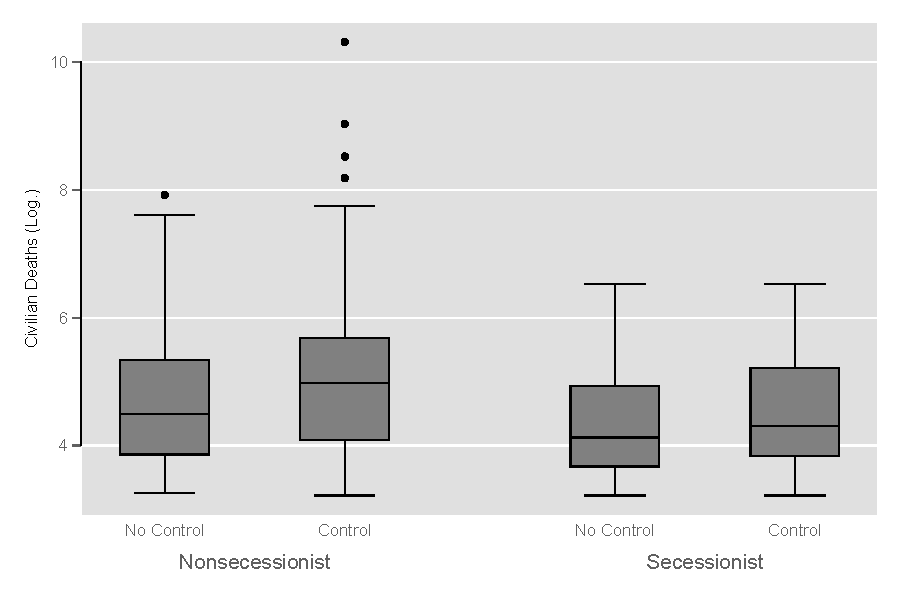
\includegraphics[width=\textwidth]{DVIVTERRSECbox.pdf}
\end{figure} 

This section gives an overview of the state of research on rebel organizations' behavior in civil war, these groups' relationship with states, and finally a relatively recent finding in the field: the distinct behavior of secessionist rebels in Figure \ref{f1}. \\ \

\begin{table}[!htbp] \centering 
	\caption{Regression Results} 
	\label{} 
	\begin{tabular}{@{\extracolsep{5pt}}lD{.}{.}{-3} } 
		\\[-1.8ex]\hline 
		\hline \\[-1.8ex] 
		& \multicolumn{1}{c}{\textit{Dependent variable:}} \\ 
		\cline{2-2} 
		\\[-1.8ex] & \multicolumn{1}{c}{womleg\_2015} \\ 
		\hline \\[-1.8ex] 
		libpct\_m & 1.146^{***} \\ 
		& (0.215) \\ 
		& \\ 
		Constant & 1.524 \\ 
		& (4.329) \\ 
		& \\ 
		\hline \\[-1.8ex] 
		Observations & \multicolumn{1}{c}{50} \\ 
		R$^{2}$ & \multicolumn{1}{c}{0.371} \\ 
		Adjusted R$^{2}$ & \multicolumn{1}{c}{0.358} \\ 
		Residual Std. Error & \multicolumn{1}{c}{5.616 (df = 48)} \\ 
		F Statistic & \multicolumn{1}{c}{28.280$^{***}$ (df = 1; 48)} \\ 
		\hline 
		\hline \\[-1.8ex] 
		\textit{Note:}  & \multicolumn{1}{r}{$^{*}$p$<$0.1; $^{**}$p$<$0.05; $^{***}$p$<$0.01} \\ 
	\end{tabular} 
\end{table} 

While this can be attributed to the pivot in security studies from great power competition to intrastate conflict, it has also been furthered by the accumulation of more precise data and refinement of methods, see Table.

\pagebreak 

\noindent Purely rationalist and structuralist explanations \cite{Cunningham2009} are still prevalent like \cite{Berman2008} argue, but conflict scholars now increasingly argue that there is a link between compliance with international norms of statehood and the behavior of certain non-state actors \citep{Stewart2018,Cunningham2009,Fazal2019}: Just like Franklin on behalf of the Second Continental Congress \citep[433--435]{Coggins2011}, rebel groups that wish to secede from an existing nation-state to determine their own destiny mimic states' behavior in the international system and towards the domestic population in order to garner recognition and material support.

\pagebreak

\section{References}
\bibliographystyle{Chicago16}
\begingroup
\renewcommand{\section}[2]{}
\bibliography{FinalPaper}
\endgroup

\end{document}